\documentclass[a4paperpaper,]{article}
\usepackage{lmodern}
\usepackage{svg}
\usepackage{amssymb,amsmath}
\usepackage{ifxetex,ifluatex}
\usepackage{fixltx2e} % provides \textsubscript
\ifnum 0\ifxetex 1\fi\ifluatex 1\fi=0 % if pdftex
  \usepackage[T1]{fontenc}
  \usepackage[utf8]{inputenc}
\else % if luatex or xelatex
  \ifxetex
    \usepackage{mathspec}
  \else
    \usepackage{fontspec}
  \fi
  \defaultfontfeatures{Ligatures=TeX,Scale=MatchLowercase}
\fi
% use upquote if available, for straight quotes in verbatim environments
\IfFileExists{upquote.sty}{\usepackage{upquote}}{}
% use microtype if available
\IfFileExists{microtype.sty}{%
\usepackage{microtype}
\UseMicrotypeSet[protrusion]{basicmath} % disable protrusion for tt fonts
}{}
\usepackage[a4paper,margin=2cm]{geometry}
\usepackage[unicode=true]{hyperref}
\hypersetup{
            pdftitle={The NIPS Experiment},
            pdfborder={0 0 0},
            breaklinks=true}
\urlstyle{same}  % don't use monospace font for urls
\usepackage{natbib}
\bibliographystyle{plainnat}
\usepackage{color}
\usepackage{fancyvrb}
\newcommand{\VerbBar}{|}
\newcommand{\VERB}{\Verb[commandchars=\\\{\}]}
\DefineVerbatimEnvironment{Highlighting}{Verbatim}{commandchars=\\\{\}}
% Add ',fontsize=\small' for more characters per line
\newenvironment{Shaded}{}{}
\newcommand{\AlertTok}[1]{\textcolor[rgb]{1.00,0.00,0.00}{\textbf{#1}}}
\newcommand{\AnnotationTok}[1]{\textcolor[rgb]{0.38,0.63,0.69}{\textbf{\textit{#1}}}}
\newcommand{\AttributeTok}[1]{\textcolor[rgb]{0.49,0.56,0.16}{#1}}
\newcommand{\BaseNTok}[1]{\textcolor[rgb]{0.25,0.63,0.44}{#1}}
\newcommand{\BuiltInTok}[1]{#1}
\newcommand{\CharTok}[1]{\textcolor[rgb]{0.25,0.44,0.63}{#1}}
\newcommand{\CommentTok}[1]{\textcolor[rgb]{0.38,0.63,0.69}{\textit{#1}}}
\newcommand{\CommentVarTok}[1]{\textcolor[rgb]{0.38,0.63,0.69}{\textbf{\textit{#1}}}}
\newcommand{\ConstantTok}[1]{\textcolor[rgb]{0.53,0.00,0.00}{#1}}
\newcommand{\ControlFlowTok}[1]{\textcolor[rgb]{0.00,0.44,0.13}{\textbf{#1}}}
\newcommand{\DataTypeTok}[1]{\textcolor[rgb]{0.56,0.13,0.00}{#1}}
\newcommand{\DecValTok}[1]{\textcolor[rgb]{0.25,0.63,0.44}{#1}}
\newcommand{\DocumentationTok}[1]{\textcolor[rgb]{0.73,0.13,0.13}{\textit{#1}}}
\newcommand{\ErrorTok}[1]{\textcolor[rgb]{1.00,0.00,0.00}{\textbf{#1}}}
\newcommand{\ExtensionTok}[1]{#1}
\newcommand{\FloatTok}[1]{\textcolor[rgb]{0.25,0.63,0.44}{#1}}
\newcommand{\FunctionTok}[1]{\textcolor[rgb]{0.02,0.16,0.49}{#1}}
\newcommand{\ImportTok}[1]{#1}
\newcommand{\InformationTok}[1]{\textcolor[rgb]{0.38,0.63,0.69}{\textbf{\textit{#1}}}}
\newcommand{\KeywordTok}[1]{\textcolor[rgb]{0.00,0.44,0.13}{\textbf{#1}}}
\newcommand{\NormalTok}[1]{#1}
\newcommand{\OperatorTok}[1]{\textcolor[rgb]{0.40,0.40,0.40}{#1}}
\newcommand{\OtherTok}[1]{\textcolor[rgb]{0.00,0.44,0.13}{#1}}
\newcommand{\PreprocessorTok}[1]{\textcolor[rgb]{0.74,0.48,0.00}{#1}}
\newcommand{\RegionMarkerTok}[1]{#1}
\newcommand{\SpecialCharTok}[1]{\textcolor[rgb]{0.25,0.44,0.63}{#1}}
\newcommand{\SpecialStringTok}[1]{\textcolor[rgb]{0.73,0.40,0.53}{#1}}
\newcommand{\StringTok}[1]{\textcolor[rgb]{0.25,0.44,0.63}{#1}}
\newcommand{\VariableTok}[1]{\textcolor[rgb]{0.10,0.09,0.49}{#1}}
\newcommand{\VerbatimStringTok}[1]{\textcolor[rgb]{0.25,0.44,0.63}{#1}}
\newcommand{\WarningTok}[1]{\textcolor[rgb]{0.38,0.63,0.69}{\textbf{\textit{#1}}}}
\IfFileExists{parskip.sty}{%
\usepackage{parskip}
}{% else
\setlength{\parindent}{0pt}
\setlength{\parskip}{6pt plus 2pt minus 1pt}
}
\setcounter{secnumdepth}{5}


% set default figure placement to htbp
\makeatletter

\def\fps@figure{htbp}
\makeatother
\usepackage{graphicx}



\usepackage{amssymb} 
\usepackage{enumitem}
\usepackage{xcolor}
\usepackage{lipsum}
\usepackage{titlesec}

\providecommand{\tightlist}{%
  \setlength{\itemsep}{0pt}\setlength{\parskip}{0pt}}


\begin{document}


\title{The NIPS Experiment}

\author{Neil D. Lawrence}

\date{2015-01-30}


\maketitle

\abstract{The peer review process can be difficult to navigate for
newcomers. In this informal talk we will review the results of the NIPS
experiment, an experiment on the repeatability of peer review conducted
for the 2014 conference. We will try to keep the presentation
information to ensure questions can be asked. With luck it will give
more insight into the processes that a program committee goes through
when selecting papers.}

\newcommand{\tk}[1]{}
\newcommand{\Amatrix}{\mathbf{A}}
\newcommand{\KL}[2]{\text{KL}\left( #1\,\|\,#2 \right)}
\newcommand{\Kaast}{\kernelMatrix_{\mathbf{ \ast}\mathbf{ \ast}}}
\newcommand{\Kastu}{\kernelMatrix_{\mathbf{ \ast} \inducingVector}}
\newcommand{\Kff}{\kernelMatrix_{\mappingFunctionVector \mappingFunctionVector}}
\newcommand{\Kfu}{\kernelMatrix_{\mappingFunctionVector \inducingVector}}
\newcommand{\Kuast}{\kernelMatrix_{\inducingVector \bf\ast}}
\newcommand{\Kuf}{\kernelMatrix_{\inducingVector \mappingFunctionVector}}
\newcommand{\Kuu}{\kernelMatrix_{\inducingVector \inducingVector}}
\newcommand{\Kuui}{\Kuu^{-1}}
\newcommand{\Qaast}{\mathbf{Q}_{\bf \ast \ast}}
\newcommand{\Qastf}{\mathbf{Q}_{\ast \mappingFunction}}
\newcommand{\Qfast}{\mathbf{Q}_{\mappingFunctionVector \bf \ast}}
\newcommand{\Qff}{\mathbf{Q}_{\mappingFunctionVector \mappingFunctionVector}}
\newcommand{\aMatrix}{\mathbf{A}}
\newcommand{\aScalar}{a}
\newcommand{\aVector}{\mathbf{a}}
\newcommand{\acceleration}{a}
\newcommand{\bMatrix}{\mathbf{B}}
\newcommand{\bScalar}{b}
\newcommand{\bVector}{\mathbf{b}}
\newcommand{\basisFunc}{\phi}
\newcommand{\basisFuncVector}{\boldsymbol{ \basisFunc}}
\newcommand{\basisFunction}{\phi}
\newcommand{\basisLocation}{\mu}
\newcommand{\basisMatrix}{\boldsymbol{ \Phi}}
\newcommand{\basisScalar}{\basisFunction}
\newcommand{\basisVector}{\boldsymbol{ \basisFunction}}
\newcommand{\activationFunction}{\phi}
\newcommand{\activationMatrix}{\boldsymbol{ \Phi}}
\newcommand{\activationScalar}{\basisFunction}
\newcommand{\activationVector}{\boldsymbol{ \basisFunction}}
\newcommand{\bigO}{\mathcal{O}}
\newcommand{\binomProb}{\pi}
\newcommand{\cMatrix}{\mathbf{C}}
\newcommand{\cbasisMatrix}{\hat{\boldsymbol{ \Phi}}}
\newcommand{\cdataMatrix}{\hat{\dataMatrix}}
\newcommand{\cdataScalar}{\hat{\dataScalar}}
\newcommand{\cdataVector}{\hat{\dataVector}}
\newcommand{\centeredKernelMatrix}{\mathbf{ \MakeUppercase{\centeredKernelScalar}}}
\newcommand{\centeredKernelScalar}{b}
\newcommand{\centeredKernelVector}{\centeredKernelScalar}
\newcommand{\centeringMatrix}{\mathbf{H}}
\newcommand{\chiSquaredDist}[2]{\chi_{#1}^{2}\left(#2\right)}
\newcommand{\chiSquaredSamp}[1]{\chi_{#1}^{2}}
\newcommand{\conditionalCovariance}{\boldsymbol{ \Sigma}}
\newcommand{\coregionalizationMatrix}{\mathbf{B}}
\newcommand{\coregionalizationScalar}{b}
\newcommand{\coregionalizationVector}{\mathbf{ \coregionalizationScalar}}
\newcommand{\covDist}[2]{\text{cov}_{#2}\left(#1\right)}
\newcommand{\covSamp}[1]{\text{cov}\left(#1\right)}
\newcommand{\covarianceScalar}{c}
\newcommand{\covarianceVector}{\mathbf{ \covarianceScalar}}
\newcommand{\covarianceMatrix}{\mathbf{C}}
\newcommand{\covarianceMatrixTwo}{\boldsymbol{ \Sigma}}
\newcommand{\croupierScalar}{s}
\newcommand{\croupierVector}{\mathbf{ \croupierScalar}}
\newcommand{\croupierMatrix}{\mathbf{ \MakeUppercase{\croupierScalar}}}
\newcommand{\dataDim}{p}
\newcommand{\dataIndex}{i}
\newcommand{\dataIndexTwo}{j}
\newcommand{\dataMatrix}{\mathbf{Y}}
\newcommand{\dataScalar}{y}
\newcommand{\dataSet}{\mathcal{D}}
\newcommand{\dataStd}{\sigma}
\newcommand{\dataVector}{\mathbf{ \dataScalar}}
\newcommand{\decayRate}{d}
\newcommand{\degreeMatrix}{\mathbf{ \MakeUppercase{\degreeScalar}}}
\newcommand{\degreeScalar}{d}
\newcommand{\degreeVector}{\mathbf{ \degreeScalar}}
\newcommand{\diag}[1]{\text{diag}\left(#1\right)}
\newcommand{\diagonalMatrix}{\mathbf{D}}
\newcommand{\diff}[2]{\frac{\text{d}#1}{\text{d}#2}}
\newcommand{\diffTwo}[2]{\frac{\text{d}^2#1}{\text{d}#2^2}}
\newcommand{\displacement}{x}
\newcommand{\displacementVector}{\textbf{\displacement}}
\newcommand{\distanceMatrix}{\mathbf{ \MakeUppercase{\distanceScalar}}}
\newcommand{\distanceScalar}{d}
\newcommand{\distanceVector}{\mathbf{ \distanceScalar}}
\newcommand{\eigenvaltwo}{\ell}
\newcommand{\eigenvaltwoMatrix}{\mathbf{L}}
\newcommand{\eigenvaltwoVector}{\mathbf{l}}
\newcommand{\eigenvalue}{\lambda}
\newcommand{\eigenvalueMatrix}{\boldsymbol{ \Lambda}}
\newcommand{\eigenvalueVector}{\boldsymbol{ \lambda}}
\newcommand{\eigenvector}{\mathbf{ \eigenvectorScalar}}
\newcommand{\eigenvectorMatrix}{\mathbf{U}}
\newcommand{\eigenvectorScalar}{u}
\newcommand{\eigenvectwo}{\mathbf{v}}
\newcommand{\eigenvectwoMatrix}{\mathbf{V}}
\newcommand{\eigenvectwoScalar}{v}
\newcommand{\entropy}[1]{\mathcal{H}\left(#1\right)}
\newcommand{\errorFunction}{E}
\newcommand{\expDist}[2]{\left<#1\right>_{#2}}
\newcommand{\expSamp}[1]{\left<#1\right>}
\newcommand{\expectation}[1]{\left\langle #1 \right\rangle }
\newcommand{\expectationDist}[2]{\left\langle #1 \right\rangle _{#2}}
\newcommand{\expectedDistanceMatrix}{\mathcal{D}}
\newcommand{\eye}{\mathbf{I}}
\newcommand{\fantasyDim}{r}
\newcommand{\fantasyMatrix}{\mathbf{ \MakeUppercase{\fantasyScalar}}}
\newcommand{\fantasyScalar}{z}
\newcommand{\fantasyVector}{\mathbf{ \fantasyScalar}}
\newcommand{\featureStd}{\varsigma}
\newcommand{\gammaCdf}[3]{\mathcal{GAMMA CDF}\left(#1|#2,#3\right)}
\newcommand{\gammaDist}[3]{\mathcal{G}\left(#1|#2,#3\right)}
\newcommand{\gammaSamp}[2]{\mathcal{G}\left(#1,#2\right)}
\newcommand{\gaussianDist}[3]{\mathcal{N}\left(#1|#2,#3\right)}
\newcommand{\gaussianSamp}[2]{\mathcal{N}\left(#1,#2\right)}
\newcommand{\uniformDist}[3]{\mathcal{U}\left(#1|#2,#3\right)}
\newcommand{\uniformSamp}[2]{\mathcal{U}\left(#1,#2\right)}
\newcommand{\given}{|}
\newcommand{\half}{\frac{1}{2}}
\newcommand{\heaviside}{H}
\newcommand{\hiddenMatrix}{\mathbf{ \MakeUppercase{\hiddenScalar}}}
\newcommand{\hiddenScalar}{h}
\newcommand{\hiddenVector}{\mathbf{ \hiddenScalar}}
\newcommand{\identityMatrix}{\eye}
\newcommand{\inducingInputScalar}{z}
\newcommand{\inducingInputVector}{\mathbf{ \inducingInputScalar}}
\newcommand{\inducingInputMatrix}{\mathbf{Z}}
\newcommand{\inducingScalar}{u}
\newcommand{\inducingVector}{\mathbf{ \inducingScalar}}
\newcommand{\inducingMatrix}{\mathbf{U}}
\newcommand{\inlineDiff}[2]{\text{d}#1/\text{d}#2}
\newcommand{\inputDim}{q}
\newcommand{\inputMatrix}{\mathbf{X}}
\newcommand{\inputScalar}{x}
\newcommand{\inputSpace}{\mathcal{X}}
\newcommand{\inputVals}{\inputVector}
\newcommand{\inputVector}{\mathbf{ \inputScalar}}
\newcommand{\iterNum}{k}
\newcommand{\kernel}{\kernelScalar}
\newcommand{\kernelMatrix}{\mathbf{K}}
\newcommand{\kernelScalar}{k}
\newcommand{\kernelVector}{\mathbf{ \kernelScalar}}
\newcommand{\kff}{\kernelScalar_{\mappingFunction \mappingFunction}}
\newcommand{\kfu}{\kernelVector_{\mappingFunction \inducingScalar}}
\newcommand{\kuf}{\kernelVector_{\inducingScalar \mappingFunction}}
\newcommand{\kuu}{\kernelVector_{\inducingScalar \inducingScalar}}
\newcommand{\lagrangeMultiplier}{\lambda}
\newcommand{\lagrangeMultiplierMatrix}{\boldsymbol{ \Lambda}}
\newcommand{\lagrangian}{L}
\newcommand{\laplacianFactor}{\mathbf{ \MakeUppercase{\laplacianFactorScalar}}}
\newcommand{\laplacianFactorScalar}{m}
\newcommand{\laplacianFactorVector}{\mathbf{ \laplacianFactorScalar}}
\newcommand{\laplacianMatrix}{\mathbf{L}}
\newcommand{\laplacianScalar}{\ell}
\newcommand{\laplacianVector}{\mathbf{ \ell}}
\newcommand{\latentDim}{q}
\newcommand{\latentDistanceMatrix}{\boldsymbol{ \Delta}}
\newcommand{\latentDistanceScalar}{\delta}
\newcommand{\latentDistanceVector}{\boldsymbol{ \delta}}
\newcommand{\latentForce}{f}
\newcommand{\latentFunction}{u}
\newcommand{\latentFunctionVector}{\mathbf{ \latentFunction}}
\newcommand{\latentFunctionMatrix}{\mathbf{ \MakeUppercase{\latentFunction}}}
\newcommand{\latentIndex}{j}
\newcommand{\latentScalar}{z}
\newcommand{\latentVector}{\mathbf{ \latentScalar}}
\newcommand{\latentMatrix}{\mathbf{Z}}
\newcommand{\learnRate}{\eta}
\newcommand{\lengthScale}{\ell}
\newcommand{\rbfWidth}{\ell}
\newcommand{\likelihoodBound}{\mathcal{L}}
\newcommand{\likelihoodFunction}{L}
\newcommand{\locationScalar}{\mu}
\newcommand{\locationVector}{\boldsymbol{ \locationScalar}}
\newcommand{\locationMatrix}{\mathbf{M}}
\newcommand{\variance}[1]{\text{var}\left( #1 \right)}
\newcommand{\mappingFunction}{f}
\newcommand{\mappingFunctionMatrix}{\mathbf{F}}
\newcommand{\mappingFunctionTwo}{g}
\newcommand{\mappingFunctionTwoMatrix}{\mathbf{G}}
\newcommand{\mappingFunctionTwoVector}{\mathbf{ \mappingFunctionTwo}}
\newcommand{\mappingFunctionVector}{\mathbf{ \mappingFunction}}
\newcommand{\scaleScalar}{s}
\newcommand{\mappingScalar}{w}
\newcommand{\mappingVector}{\mathbf{ \mappingScalar}}
\newcommand{\mappingMatrix}{\mathbf{W}}
\newcommand{\mappingScalarTwo}{v}
\newcommand{\mappingVectorTwo}{\mathbf{ \mappingScalarTwo}}
\newcommand{\mappingMatrixTwo}{\mathbf{V}}
\newcommand{\maxIters}{K}
\newcommand{\meanMatrix}{\mathbf{M}}
\newcommand{\meanScalar}{\mu}
\newcommand{\meanTwoMatrix}{\mathbf{M}}
\newcommand{\meanTwoScalar}{m}
\newcommand{\meanTwoVector}{\mathbf{ \meanTwoScalar}}
\newcommand{\meanVector}{\boldsymbol{ \meanScalar}}
\newcommand{\mrnaConcentration}{m}
\newcommand{\naturalFrequency}{\omega}
\newcommand{\neighborhood}[1]{\mathcal{N}\left( #1 \right)}
\newcommand{\neilurl}{http://inverseprobability.com/}
\newcommand{\noiseMatrix}{\boldsymbol{ E}}
\newcommand{\noiseScalar}{\epsilon}
\newcommand{\noiseVector}{\boldsymbol{ \epsilon}}
\newcommand{\noiseStd}{\sigma}
\newcommand{\norm}[1]{\left\Vert #1 \right\Vert}
\newcommand{\normalizedLaplacianMatrix}{\hat{\mathbf{L}}}
\newcommand{\normalizedLaplacianScalar}{\hat{\ell}}
\newcommand{\normalizedLaplacianVector}{\hat{\mathbf{ \ell}}}
\newcommand{\numActive}{m}
\newcommand{\numBasisFunc}{m}
\newcommand{\numComponents}{m}
\newcommand{\numComps}{K}
\newcommand{\numData}{n}
\newcommand{\numFeatures}{K}
\newcommand{\numHidden}{h}
\newcommand{\numInducing}{m}
\newcommand{\numLayers}{\ell}
\newcommand{\numNeighbors}{K}
\newcommand{\numSequences}{s}
\newcommand{\numSuccess}{s}
\newcommand{\numTasks}{m}
\newcommand{\numTime}{T}
\newcommand{\numTrials}{S}
\newcommand{\outputIndex}{j}
\newcommand{\paramVector}{\boldsymbol{ \theta}}
\newcommand{\parameterMatrix}{\boldsymbol{ \Theta}}
\newcommand{\parameterScalar}{\theta}
\newcommand{\parameterVector}{\boldsymbol{ \parameterScalar}}
\newcommand{\partDiff}[2]{\frac{\partial#1}{\partial#2}}
\newcommand{\precisionScalar}{j}
\newcommand{\precisionVector}{\mathbf{ \precisionScalar}}
\newcommand{\precisionMatrix}{\mathbf{J}}
\newcommand{\pseudotargetScalar}{\widetilde{y}}
\newcommand{\pseudotargetVector}{\mathbf{ \pseudotargetScalar}}
\newcommand{\pseudotargetMatrix}{\mathbf{ \widetilde{Y}}}
\newcommand{\rank}[1]{\text{rank}\left(#1\right)}
\newcommand{\rayleighDist}[2]{\mathcal{R}\left(#1|#2\right)}
\newcommand{\rayleighSamp}[1]{\mathcal{R}\left(#1\right)}
\newcommand{\responsibility}{r}
\newcommand{\rotationScalar}{r}
\newcommand{\rotationVector}{\mathbf{ \rotationScalar}}
\newcommand{\rotationMatrix}{\mathbf{R}}
\newcommand{\sampleCovScalar}{s}
\newcommand{\sampleCovVector}{\mathbf{ \sampleCovScalar}}
\newcommand{\sampleCovMatrix}{\mathbf{s}}
\newcommand{\scalarProduct}[2]{\left\langle{#1},{#2}\right\rangle}
\newcommand{\sign}[1]{\text{sign}\left(#1\right)}
\newcommand{\sigmoid}[1]{\sigma\left(#1\right)}
\newcommand{\singularvalue}{\ell}
\newcommand{\singularvalueMatrix}{\mathbf{L}}
\newcommand{\singularvalueVector}{\mathbf{l}}
\newcommand{\sorth}{\mathbf{u}}
\newcommand{\spar}{\lambda}
\newcommand{\trace}[1]{\text{tr}\left(#1\right)}
\newcommand{\BasalRate}{B}
\newcommand{\DampingCoefficient}{C}
\newcommand{\DecayRate}{D}
\newcommand{\Displacement}{X}
\newcommand{\LatentForce}{F}
\newcommand{\Mass}{M}
\newcommand{\Sensitivity}{S}
\newcommand{\basalRate}{b}
\newcommand{\dampingCoefficient}{c}
\newcommand{\mass}{m}
\newcommand{\sensitivity}{s}
\newcommand{\springScalar}{\kappa}
\newcommand{\springVector}{\boldsymbol{ \kappa}}
\newcommand{\springMatrix}{\boldsymbol{ \mathcal{K}}}
\newcommand{\tfConcentration}{p}
\newcommand{\tfDecayRate}{\delta}
\newcommand{\tfMrnaConcentration}{f}
\newcommand{\tfVector}{\mathbf{ \tfConcentration}}
\newcommand{\velocity}{v}
\newcommand{\sufficientStatsScalar}{g}
\newcommand{\sufficientStatsVector}{\mathbf{ \sufficientStatsScalar}}
\newcommand{\sufficientStatsMatrix}{\mathbf{G}}
\newcommand{\switchScalar}{s}
\newcommand{\switchVector}{\mathbf{ \switchScalar}}
\newcommand{\switchMatrix}{\mathbf{S}}
\newcommand{\tr}[1]{\text{tr}\left(#1\right)}
\newcommand{\loneNorm}[1]{\left\Vert #1 \right\Vert_1}
\newcommand{\ltwoNorm}[1]{\left\Vert #1 \right\Vert_2}
\newcommand{\onenorm}[1]{\left\vert#1\right\vert_1}
\newcommand{\twonorm}[1]{\left\Vert #1 \right\Vert}
\newcommand{\vScalar}{v}
\newcommand{\vVector}{\mathbf{v}}
\newcommand{\vMatrix}{\mathbf{V}}
\newcommand{\varianceDist}[2]{\text{var}_{#2}\left( #1 \right)}
\newcommand{\vecb}[1]{\left(#1\right):}
\newcommand{\weightScalar}{w}
\newcommand{\weightVector}{\mathbf{ \weightScalar}}
\newcommand{\weightMatrix}{\mathbf{W}}
\newcommand{\weightedAdjacencyMatrix}{\mathbf{A}}
\newcommand{\weightedAdjacencyScalar}{a}
\newcommand{\weightedAdjacencyVector}{\mathbf{ \weightedAdjacencyScalar}}
\newcommand{\onesVector}{\mathbf{1}}
\newcommand{\zerosVector}{\mathbf{0}}


%%%%%%%%%% Start Body %%%%%%%%%%

\definecolor{societyColor}{RGB}{221,221,78}

\definecolor{vulnerabilityColor}{RGB}{78,221,78}

\definecolor{enfranchisementColor}{RGB}{78,221,78}

\definecolor{individualColor}{RGB}{221,78,78}

The NIPS experiment was an experiment to determine the consistency of
the review process. After receiving papers we selected 10\% that would
be independently rereviewed. The idea was to determine how consistent
the decisions between the two sets of independent papers would be. In
2014 NIPS received 1678 submissions and we selected 170 for the
experiment. These papers are referred to below as `duplicated papers'.

To run the experiment we created two separate committees within the NIPS
program committee. The idea was that the two separate committees would
review each duplicated paper independently and results compared.

\hypertarget{neurips-in-numbers}{%
\subsection{NeurIPS in Numbers}\label{neurips-in-numbers}}

\begin{flushright}
[\href{https://github.com/lawrennd/talks/edit/gh-pages/_neurips/includes/neurips-in-numbers.md}{edit}]
\end{flushright}

In 2014 the NeurIPS conference had 1474 active reviewers (up from 1133
in 2013), 92 area chairs (up from 67 in 2013) and two program chairs,
myself and Corinna Cortes.

The conference received 1678 submissions and presented 414 accepted
papers, of which 20 were presented as talks in the single track session,
62 were presented as spotlights and 331 papers were presented as
posters. Of the 1678 submissions, 19 papers were rejected without
review.

\hypertarget{the-neurips-experiment}{%
\subsection{The NeurIPS Experiment}\label{the-neurips-experiment}}

The objective of the NeurIPS experiment was to determine how consistent
the process of peer review is. One way of phraising this question is to
ask: what would happen to submitted papers in the conference if the
process was independently rerun?

For the 2014 conference, to explore this question, we selected
\(\approx 10\%\) of submitted papers to be reviewed twice, by
independent committees. This led to 170 papers being selected from the
conference for dual reviewing. For these papers the program committee
was divided into two. Reviewers were placed randomly on one side of the
committee or the other. For Program Chairs we also engaged in some
manual selection to ensure we had expert coverage in all the conference
areas on both side of the committee.

\hypertarget{timeline-for-neurips}{%
\subsection{Timeline for NeurIPS}\label{timeline-for-neurips}}

\begin{flushright}
[\href{https://github.com/lawrennd/talks/edit/gh-pages/_neurips/includes/neurips-timeline.md}{edit}]
\end{flushright}

\paragraph{AC recruitment (3 waves)}

Chairing a conference starts with recruitment of the program committee,
which is usually done in a few stages. The primary task is to recruit
the area chairs. We sent out our program committee invites in three
waves.

\begin{itemize}
\tightlist
\item
  17/02/2014
\item
  08/03/2014
\item
  09/04/2014
\end{itemize}

By recruiting area chairs first, you can involve them in recruiting
reviewers. We requested names of reviewers from ACs in two waves.

\begin{itemize}
\tightlist
\item
  25/03/2014
\item
  11/04/2014
\end{itemize}

In 2014, this wasn't enough to obtain the requisite number of reviewers,
so we used additional approaches. These included lists of previous
NeurIPS authors. For each individual we were looking for at least two
previous papers published or papers published at NeurIPS and other
leading ML venues like ICML, AISTATS, COLT, UAI etc. We made extensive
use of \href{https://dblp.uni-trier.de/}{DBLP} for verifying potential
reviewer's publication track record.

\paragraph{Reviewer recruitment}

\begin{itemize}
\tightlist
\item
  14/04/2014
\item
  28/04/2014
\item
  09/05/2014
\item
  10/06/2014 (note this is after deadline \ldots{} lots of area chairs
  asked for reviewers after the deadline!). We invited them en-masse.
\end{itemize}

\paragraph{Decision Making Timeline}

\begin{itemize}
\tightlist
\item
  06/06/2014 Submission Deadline
\item
  12/06/2014 Bidding Open For Area Chairs (this was \emph{delayed} by
  CMT issues)
\item
  17/06/2014 Bidding Open For Reviewers
\item
  01/07/2014 Start Reviewing
\item
  21/07/2014 Reviewing deadline
\item
  04/08/2014 Reviews to Authors
\item
  11/08/2014 Author Rebuttal Due
\item
  25/08/2014 Teleconferences Begin
\item
  30/08/2014 Teleconferences End
\item
  1/09/2014 Preliminary Decisions Made
\item
  9/09/2014 Decisions Sent to Authors
\end{itemize}

\hypertarget{speculation}{%
\subsection{Speculation}\label{speculation}}

\begin{flushright}
[\href{https://github.com/lawrennd/talks/edit/gh-pages/_neurips/includes/neurips-experiment-speculation.md}{edit}]
\end{flushright}

With the help of \href{http://nicolofusi.com/}{Nicolo Fusi},
\href{http://blog.scicast.org/tag/charles-twardy/}{Charles Twardy} and
the entire Scicast team we launched
\href{https://scicast.org/\#!/questions/1083/trades/create/power}{a
Scicast question}~a week before the results were revealed. The comment
thread for that question already had
\href{https://scicast.org/\#!/questions/1083/comments/power}{an amount
of interesting comment}~before the conference. Just for informational
purposes before we began reviewing Corinna forecast this figure would be
25\% and I forecast it would be 20\%. The box plot summary of
predictions from Scicast is below.

\begin{figure}[htb]
\begin{center}
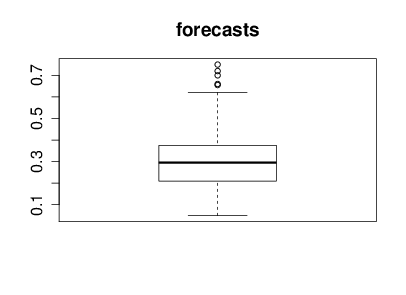
\includegraphics[width=0.40\textwidth]{https://inverseprobability.com/talks/slides/diagrams//neurips/scicast-forecast.png}
\end{center}


\caption{Summary forecast from those that responded to a scicast question about how consistent the decision making was.}
\label{scicast-forecast}
\end{figure}

\hypertarget{neurips-experiment-results}{%
\subsection{NeurIPS Experiment
Results}\label{neurips-experiment-results}}

\begin{flushright}
[\href{https://github.com/lawrennd/talks/edit/gh-pages/_neurips/includes/neurips-experiment-results.md}{edit}]
\end{flushright}

The final results of the experiment were as follows. From 170 papers 4
had to be withdrawn or were rejected without completing the review
process, for the remainder, the `confusion matrix' for the two
committee's decisions is below.

Committee 1

Accept

Reject

Committee 2

Accept

22

22

Reject

21

101

4 papers rejected or withdrawn without review.

\hypertarget{summarizing-the-table}{%
\subsection{Summarizing the Table}\label{summarizing-the-table}}

There are a few ways of summarizing the numbers in this table as percent
or probabilities. First of all, the inconsistency, the proportion of
decisions that were not the same across the two committees. The
decisions were inconsistent for 43 out of 166 papers or 0.259 as a
proportion. This number is perhaps a natural way of summarizing the
figures if you are submitting your paper and wish to know an estimate of
what the probability is that your paper would have different decisons
according to the different committes. Secondly, the accept precision: if
you are attending the conference and looking at any given paper, then
you might want to know the probability that the paper would have been
rejected in an independent rerunning of the conference. We can estimate
this for Committee 1's conference as 22/(22 + 22) = 0.5 (50\%) and for
Committee 2's conference as 21/(22+21) = 0.49 (49\%). Averaging the two
estimates gives us 49.5\%. Finally, the reject precision: if your paper
was rejected from the conference, you might like an estimate of the
probability that the same paper would be rejected again if the review
process had been independently rerun. That estimate is 101/(22+101) =
0.82 (82\%) for Committee 1 and 101/(21+101)=0.83 (83\%) for Committee
2, or on average 82.5\%. A final quality estimate might be the ratio of
consistent accepts to consistent rejects, or the agreed accept rate,
22/123 = 0.18 (18\%).

\begin{itemize}
\tightlist
\item
  \emph{inconsistency}: 43/166 = \textbf{0.259}

  \begin{itemize}
  \tightlist
  \item
    proportion of decisions that were not the same
  \end{itemize}
\item
  \emph{accept precision} \(0.5 \times 22/44\) + \(0.5 \times 21/43\) =
  \textbf{0.495}

  \begin{itemize}
  \tightlist
  \item
    probability any accepted paper would be rejected in a rerunning
  \end{itemize}
\item
  \emph{reject precision} = \(0.5\times 101/(22+101)\) +
  \(0.5\times 101/(21 + 101)\) = \textbf{0.175}

  \begin{itemize}
  \tightlist
  \item
    probability any rejected paper would be rejected in a rerunning
  \end{itemize}
\item
  \emph{agreed accept rate} = 22/101 = \textbf{0.218}
\item
  ratio between aggreed accepted papers and agreed rejected papers.
\end{itemize}

\hypertarget{reaction-after-experiment}{%
\subsection{Reaction After Experiment}\label{reaction-after-experiment}}

\begin{flushright}
[\href{https://github.com/lawrennd/talks/edit/gh-pages/_neurips/includes/neurips-experiment-reaction.md}{edit}]
\end{flushright}

There seems to have been a lot of discussion of the result, both at the
conference and on bulletin boards since. Such discussion is to be
encouraged, and for ease of memory, it is worth pointing out that the
approximate proportions of papers in each category can be nicely divided
in to eigths as follows. Accept-Accept 1 in 8 papers, Accept-Reject 3 in
8 papers, Reject-Reject, 5 in 8 papers. This makes the statistics we've
computed above: inconsistency 1 in 4 (25\%) accept precision 1 in 2
(50\%) reject precision 5 in 6 (83\%) and agreed accept rate of 1 in 6
(20\%). This compares with the accept rate of 1 in 4.

\begin{itemize}
\item
  Public reaction after experiment
  \href{http://inverseprobability.com/2015/01/16/blogs-on-the-nips-experiment/}{documented
  here}
\item
  \href{http://inverseprobability.com/2014/07/01/open-data-science/}{Open
  Data Science} (see Heidelberg Meeting)
\item
  NIPS was run in a very open way.
  \href{https://github.com/sods/conference}{Code} and
  \href{http://inverseprobability.com/2014/12/16/the-nips-experiment/}{blog
  posts} all available!
\item
  Reaction triggered by
  \href{http://blog.mrtz.org/2014/12/15/the-nips-experiment.html}{this
  blog post}.
\end{itemize}

Much of the discussion speculates on the number of consistent accepts in
the process (using the main conference accept rate as a proxy). It
therefore produces numbers that don't match ours above. This is because
the computed accept rate of the individual committees is different from
that of the main conference. This could be due to a bias for the
duplicated papers, or statistical sampling error. We look at these
questions below. First, to get the reader primed for thinking about
these numbers we discuss some context for placing these numbers.

\hypertarget{a-random-committee-25}\label{a-random-committee-25}}

\begin{flushright}
[\href{https://github.com/lawrennd/talks/edit/gh-pages/_neurips/includes/neurips-experiment-random-committee.md}{edit}]
\end{flushright}

The first context we can place around the numbers is what would have
happened at the `Random Conference' where we simply accept a quarter of
papers at random. In this NIPS the expected numbers of accepts would
then have been:

Committee 1

Accept

Reject

Committee 2

Accept

10.4 (1 in 16)

31.1 (3 in 16)

Reject

31.1 (3 in 16)

93.4 (9 in 16)

And for this set up we would expect \emph{inconsistency} of 3 in 8
(37.5\%) \emph{accept precision} of 1 in 4 (25\%) and a \emph{reject
precision} of 3 in 4 (75\%) and a \emph{agreed accept rate} of 1 in 10
(10\%). The actual committee made improvements on these numbers, in
particular the accept precision was markedly better with 50\%: twice as
many consistent accept decisions were made than would be expected if the
process had been performed at random and only around two thirds as many
inconsistent decisions were made as would have been expected if
decisions were made at random. However, we should treat all these
figures with some skepticism until we've performed some estimate of the
uncertainty associated with them.

\hypertarget{stats-for-random-committee}{%
\subsection{Stats for Random
Committee}\label{stats-for-random-committee}}

\begin{itemize}
\tightlist
\item
  For random committee we expect:

  \begin{itemize}
  \tightlist
  \item
    \emph{inconsistency} of 3 in 8 (37.5\%)
  \item
    \emph{accept precision} of 1 in 4 (25\%)
  \item
    \emph{reject precision} of 3 in 4 (75\%) and a
  \item
    \emph{agreed accept rate} of 1 in 10 (10\%).
  \end{itemize}
\end{itemize}

Actual committee's accept precision markedly better with 50\% accept
precision.

\hypertarget{uncertainty-accept-rate}{%
\subsection{Uncertainty: Accept Rate}\label{uncertainty-accept-rate}}

To get a handle on the uncertainty around these numbers we'll start by
making use of the (binomial
distribution){[}http://en.wikipedia.org/wiki/Binomial\_distribution{]}.
First, let's explore the fact that for the overall conference the accept
rate was around 23\%, but for the duplication committees the accept rate
was around 25\%. If we assume decisions are made according to a binomial
distribution, then is the accept rate for the duplicated papers too
high?

Note that for all our accept probability statistics we used as a
denominator the number of papers that were initially sent for review,
rather than the number where a final decision was made by the program
committee. These numbers are different because some papers are withdrawn
before the program committee makes its decision. Most commonly this
occurs after authors have seen their preliminary reviews: for NIPS 2014
we provided preliminary reviews that included paper scores. So for the
official accept probability we use the 170 as denominator. The accept
probabilities were therefore 43 out of 170 papers (25.3\%) for Committee
1 and 44 out of 170 (25.8\%) for Committee 2. This compares with the
overall conference accept rate for papers outside the duplication
process of 349 out of 1508 (23.1\%).

If the true underlying probability of an accept were actually 0.23
independent of the paper, then the probability of generating accepts for
any subset of the papers would be given by a binomial distribution.
Combining across the two committees for the duplicated papers, we see
that 87 papers in total were recommended for accept out of a total of
340 trials. out of 166 trials would be given by a binomial distribution
as depicted below.

\begin{Shaded}
\begin{Highlighting}[]
\ImportTok{import}\NormalTok{ numpy }\ImportTok{as}\NormalTok{ np}
\ImportTok{from}\NormalTok{ scipy.stats }\ImportTok{import}\NormalTok{ binom}
\ImportTok{from}\NormalTok{ IPython.display }\ImportTok{import}\NormalTok{ HTML}
\end{Highlighting}
\end{Shaded}

\begin{figure}[htb]
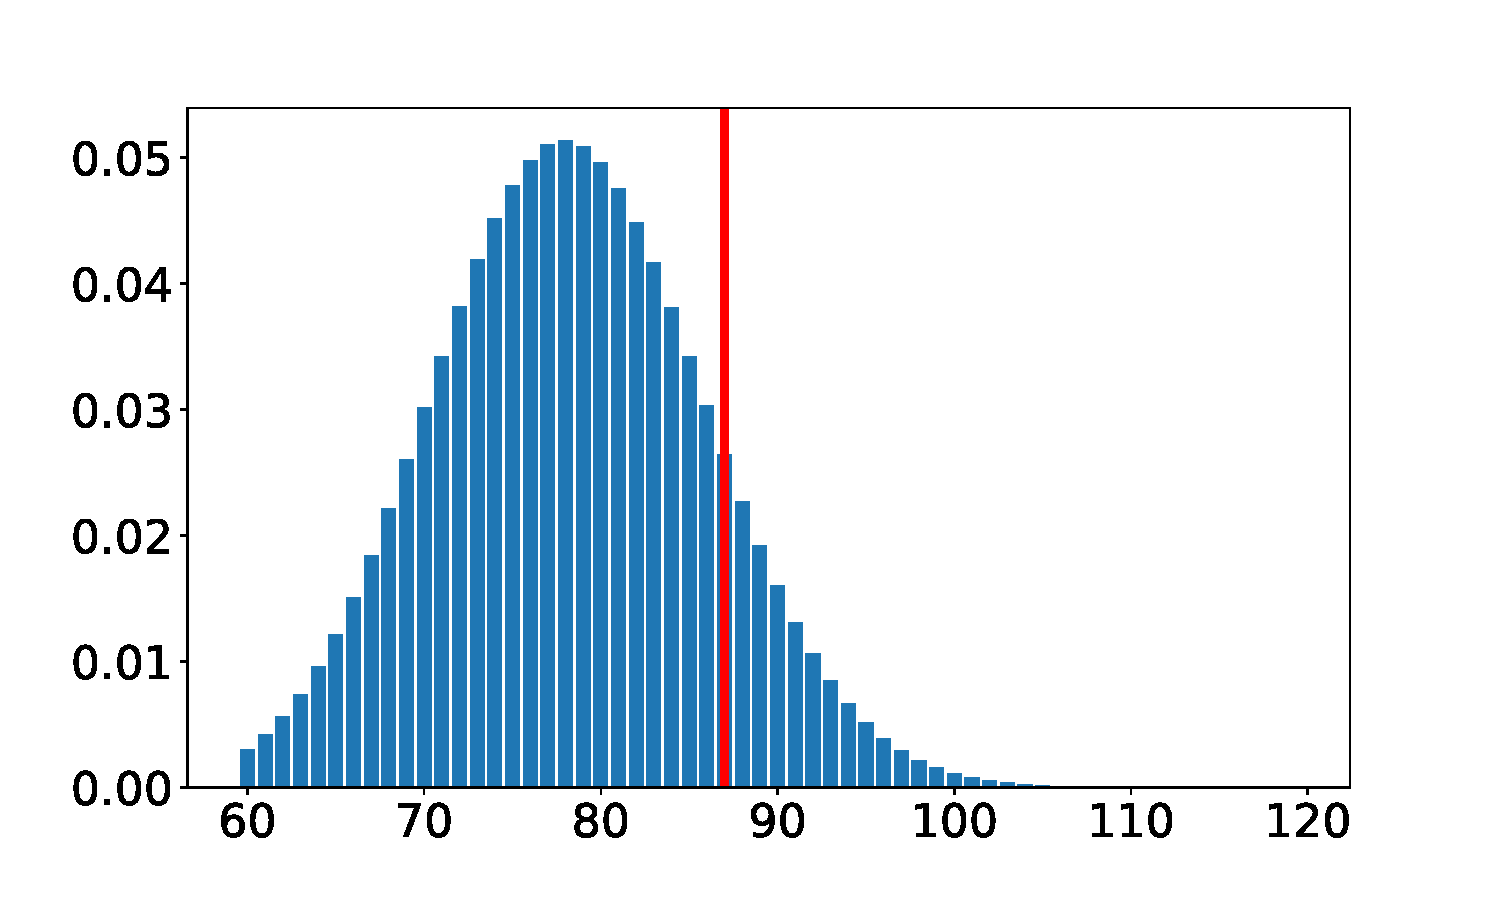
\includegraphics[width=0.70\textwidth]{https://inverseprobability.com/talks/slides/diagrams//neurips/uncertainty-accept-rate.pdf}


\caption{Number of accepted papers for $p=0.23$.}
\label{uncertainty-accept-rate}
\end{figure}

From the plot, we can see that whilst the accept rate was slightly
higher for duplicated papers it doesn't seem that we can say that it was
statistically significant that it was higher, it falls well within the
probability mass of the Binomial.

Note that Area Chairs knew which papers were duplicates, whereas
reviewers did not. Whilst we stipulated that duplicate papers should not
be any given special treatment, we cannot discount the possibility that
Area Chairs may have given slightly preferential treatment to duplicate
papers.

\hypertarget{uncertainty-accept-precision}{%
\subsection{Uncertainty: Accept
Precision}\label{uncertainty-accept-precision}}

For the accept precision, if we assume that accept decisions were drawn
according to a binomial, then the distribution for consistent accepts is
also binomial. Our best estimate of its parameter is 22/166 = 0.13
(13\%). If we had a binomial distribution with these parameters, then
the distribution of consistent accepts would be as follows.

\begin{itemize}
\tightlist
\item
  How reliable is the consistent accept score?
\end{itemize}

\begin{figure}[htb]
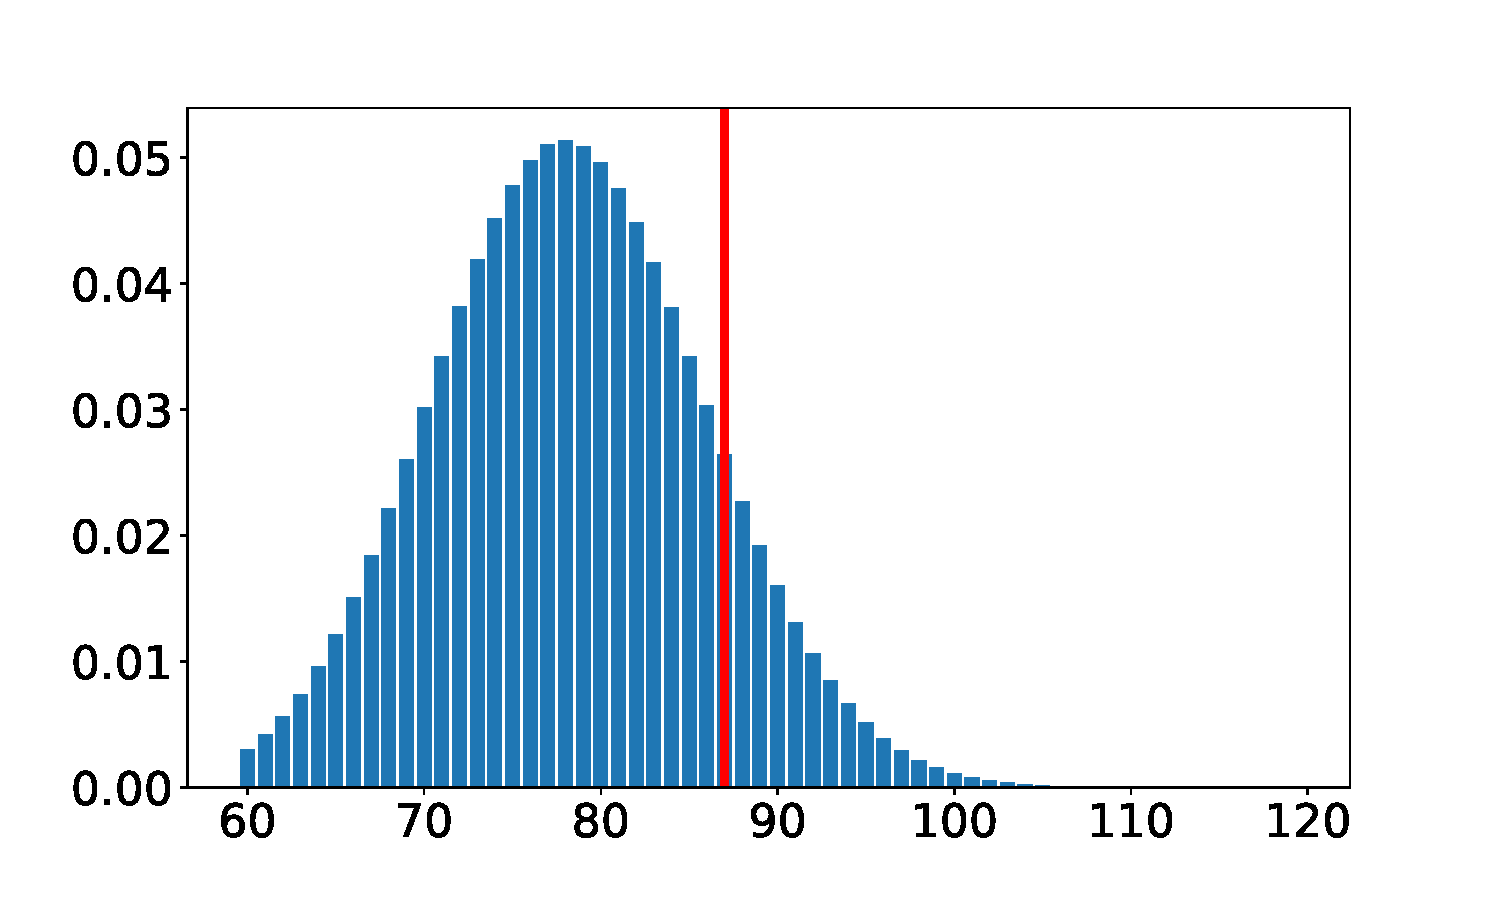
\includegraphics[width=0.70\textwidth]{https://inverseprobability.com/talks/slides/diagrams//neurips/uncertainty-accept-rate.pdf}


\caption{Number of consistent accepts given $p=0.13$.}
\label{uncertainty-accept-precision}
\end{figure}

We see immediately that there is a lot of uncertainty around this
number, for the scale of the experiment as we have it. This suggests a
more complex analysis is required to extract our estimates with
uncertainty.

\hypertarget{bayesian-analysis}{%
\subsection{Bayesian Analysis}\label{bayesian-analysis}}

Before we start the analysis, it's important to make some statements
about the aims of our modelling here. We will make some simplifying
modelling assumptions for the sake of a model that is understandable. In
particular, we are looking to get a handle on the uncertainty associated
with some of the probabilities associated with the NIPS experiment.
\href{http://inverseprobability.com/2015/01/16/blogs-on-the-nips-experiment/}{Some
preliminary analyses have already been conducted on blogs}. Those
analyses don't have access to information like paper scores etc. For
that reason we also leave out such information in this preliminary
analysis. We will focus only on the summary results from the experiment:
how many papers were consistently accepted, consistently rejected or had
inconsistent decisions. For the moment we disregard the information we
have about paper scores.

In our analysis there are three possible outcomes for each paper:
consistent accept, inconsistent decision and consistent reject. So we
need to perform the analysis with the
\href{http://en.wikipedia.org/wiki/Multinomial_distribution}{multinomial
distribution}. The multinomial is parameterized by the probabilities of
the different outcomes. These are our parameters of interest, we would
like to estimate these probabilities alongside their uncertainties. To
make a Bayesian analysis we place a prior density over these
probabilities, then we update the prior with the observed data, that
gives us a posterior density, giving us an uncertainty associated with
these probabilities.

\hypertarget{prior-density}{%
\subsubsection{Prior Density}\label{prior-density}}

Choice of prior for the multinomial is typically straightforward, the
\href{http://en.wikipedia.org/wiki/Dirichlet_distribution}{Dirichlet
density} is
\href{http://en.wikipedia.org/wiki/Conjugate_prior}{conjugate} and has
the additional advantage that its parameters can be set to ensure it is
\emph{uninformative}, i.e.~uniform across the domain of the prior.
Combination of a multinomial likelihood and a Dirichelt prior is not
new, and in this domain if we were to consider the mean the posterior
density only, then the approach is known as
\href{http://en.wikipedia.org/wiki/Additive_smoothing}{Laplace
smoothing}.

For our model we are assuming for our prior that the probabilities are
drawn from a Dirichlet as follows, \[
p \sim \text{Dir}(\alpha_1, \alpha_2, \alpha_3),
\] with \(\alpha_1=\alpha_2=\alpha_3=1\). The Dirichlet density is
conjugate to the
\href{http://en.wikipedia.org/wiki/Multinomial_distribution}{multinomial
distribution}, and we associate three different outcomes with the
multinomial. For each of the 166 papers we expect to have a consistent
accept (outcome 1), an inconsistent decision (outcome 2) or a consistent
reject (outcome 3). If the counts four outcome 1, 2 and 3 are
represented by \(k_1\), \(k_2\) and \(k_3\) and the associated
probabilities are given by \(p_1\), \(p_2\) and \(p_3\) then our model
is, \begin{align*}
\mathbf{p}|\boldsymbol{\alpha} \sim \text{Dir}(\boldsymbol{\alpha}) \\
\mathbf{k}|\mathbf{p} \sim \text{mult}(\mathbf{p}).
\end{align*} Due to the conjugacy the posterior is tractable and easily
computed as a Dirichlet (see
e.g.~\href{http://www.stat.columbia.edu/~gelman/book/}{Gelman et al}),
where the parameters of the Dirichlet are given by the original vector
from the Dirichlet prior plus the counts associated with each outcome.
\[
\mathbf{p}|\mathbf{k}, \boldsymbol{\alpha} \sim \text{Dir}(\boldsymbol{\alpha} + \mathbf{k})
\] The mean probability for each outcome is then given by, \[
\bar{p}_i = \frac{\alpha_i+k_i}{\sum_{j=1}^3(\alpha_j + k_j)}.
\] and the variance is \[
\mathrm{Var}[p_i] = \frac{(\alpha_i+k_i) (\alpha_0-\alpha_i + n + k_i)}{(\alpha_0+n)^2 (\alpha_0+n+1)},
\] where \(n\) is the number of trials (166 in our case) and
\(\alpha_0 = \sum_{i=1}^3\alpha_i\). This allows us to compute the
expected value of the probabilities and their variances under the
posterior as follows.

\begin{Shaded}
\begin{Highlighting}[]
\KeywordTok{def}\NormalTok{ posterior\_mean\_var(k, alpha):}
    \CommentTok{"""Compute the mean and variance of the Dirichlet posterior."""}
\NormalTok{    alpha\_0 }\OperatorTok{=}\NormalTok{ alpha.}\BuiltInTok{sum}\NormalTok{()}
\NormalTok{    n }\OperatorTok{=}\NormalTok{ k.}\BuiltInTok{sum}\NormalTok{()}
\NormalTok{    m }\OperatorTok{=}\NormalTok{ (k }\OperatorTok{+}\NormalTok{ alpha)}
\NormalTok{    m }\OperatorTok{/=}\NormalTok{ m.}\BuiltInTok{sum}\NormalTok{()}
\NormalTok{    v }\OperatorTok{=}\NormalTok{ (alpha}\OperatorTok{+}\NormalTok{k)}\OperatorTok{*}\NormalTok{(alpha\_0 }\OperatorTok{{-}}\NormalTok{ alpha }\OperatorTok{+}\NormalTok{ n }\OperatorTok{+}\NormalTok{ k)}\OperatorTok{/}\NormalTok{((alpha\_0}\OperatorTok{+}\NormalTok{n)}\OperatorTok{**}\DecValTok{2}\OperatorTok{*}\NormalTok{(alpha\_0}\OperatorTok{+}\NormalTok{n}\OperatorTok{+}\DecValTok{1}\NormalTok{))}
    \ControlFlowTok{return}\NormalTok{ m, v}

\NormalTok{k }\OperatorTok{=}\NormalTok{ np.asarray([}\DecValTok{22}\NormalTok{, }\DecValTok{43}\NormalTok{, }\DecValTok{101}\NormalTok{])}
\NormalTok{alpha }\OperatorTok{=}\NormalTok{ np.ones((}\DecValTok{3}\NormalTok{,))}
\NormalTok{m, v }\OperatorTok{=}\NormalTok{ posterior\_mean\_var(k, alpha)}
\NormalTok{outcome }\OperatorTok{=}\NormalTok{ [}\StringTok{\textquotesingle{}consistent accept\textquotesingle{}}\NormalTok{, }\StringTok{\textquotesingle{}inconsistent decision\textquotesingle{}}\NormalTok{, }\StringTok{\textquotesingle{}consistent reject\textquotesingle{}}\NormalTok{]}
\ControlFlowTok{for}\NormalTok{ i }\KeywordTok{in} \BuiltInTok{range}\NormalTok{(}\DecValTok{3}\NormalTok{):}
\NormalTok{    display(HTML(}\StringTok{"\textless{}h4\textgreater{}Probability of "} \OperatorTok{+}\NormalTok{ outcome[i] }\OperatorTok{+}\StringTok{\textquotesingle{} \textquotesingle{}} \OperatorTok{+} \BuiltInTok{str}\NormalTok{(m[i]) }\OperatorTok{+}  \StringTok{"+/{-}"} \OperatorTok{+} \BuiltInTok{str}\NormalTok{(}\DecValTok{2}\OperatorTok{*}\NormalTok{np.sqrt(v[i])) }\OperatorTok{+} \StringTok{"\textless{}/h4\textgreater{}"}\NormalTok{))}
\end{Highlighting}
\end{Shaded}

So we have a probability of consistent accept as \(0.136 \pm 0.06\), the
probability of inconsistent decision as \(0.260 \pm 0.09\) and
probability of consistent reject as \(0.60 \pm 0.15\). Recall that if
we'd selected papers at random (with accept rate of 1 in 4) then these
values would have been 1 in 16 (0.0625), 3 in 8 (0.375) and 9 in 16
(0.5625).

The other values we are interested in are the accept precision, reject
precision and the agreed accept rate. Computing the probability density
for these statistics is complex, because it involves
\href{http://en.wikipedia.org/wiki/Ratio_distribution}{Ratio
Distributions}. However, we can use Monte Carlo to estimate the expected
accept precision, reject precision and agreed accept rate as well as
their variances. We can use these results to give us error bars and
histograms of these statistics.

\begin{Shaded}
\begin{Highlighting}[]
\KeywordTok{def}\NormalTok{ sample\_precisions(k, alpha, num\_samps):}
    \CommentTok{"""Helper function to sample from the posterior distibution of accept, }
\CommentTok{    reject and inconsistent probabilities and compute other statistics of interest }
\CommentTok{    from the samples."""}

\NormalTok{    k }\OperatorTok{=}\NormalTok{ np.random.dirichlet(k}\OperatorTok{+}\NormalTok{alpha, size}\OperatorTok{=}\NormalTok{num\_samps)}
    \CommentTok{\# Factors of 2 appear because inconsistent decisions }
    \CommentTok{\# are being accounted for across both committees.}
\NormalTok{    ap }\OperatorTok{=} \DecValTok{2}\OperatorTok{*}\NormalTok{k[:, }\DecValTok{0}\NormalTok{]}\OperatorTok{/}\NormalTok{(}\DecValTok{2}\OperatorTok{*}\NormalTok{k[:, }\DecValTok{0}\NormalTok{]}\OperatorTok{+}\NormalTok{k[:, }\DecValTok{1}\NormalTok{])}
\NormalTok{    rp }\OperatorTok{=} \DecValTok{2}\OperatorTok{*}\NormalTok{k[:, }\DecValTok{2}\NormalTok{]}\OperatorTok{/}\NormalTok{(k[:, }\DecValTok{1}\NormalTok{]}\OperatorTok{+}\DecValTok{2}\OperatorTok{*}\NormalTok{k[:, }\DecValTok{2}\NormalTok{])}
\NormalTok{    aa }\OperatorTok{=}\NormalTok{ k[:, }\DecValTok{0}\NormalTok{]}\OperatorTok{/}\NormalTok{(k[:, }\DecValTok{0}\NormalTok{]}\OperatorTok{+}\NormalTok{k[:, }\DecValTok{2}\NormalTok{])}
    \ControlFlowTok{return}\NormalTok{ ap, rp, aa}

\NormalTok{ap, rp, aa }\OperatorTok{=}\NormalTok{ sample\_precisions(k, alpha, }\DecValTok{10000}\NormalTok{)}
\BuiltInTok{print}\NormalTok{(ap.mean(), }\StringTok{\textquotesingle{}+/{-}\textquotesingle{}}\NormalTok{, }\DecValTok{2}\OperatorTok{*}\NormalTok{np.sqrt(ap.var()))}
\BuiltInTok{print}\NormalTok{(rp.mean(), }\StringTok{\textquotesingle{}+/{-}\textquotesingle{}}\NormalTok{, }\DecValTok{2}\OperatorTok{*}\NormalTok{np.sqrt(rp.var()))}
\BuiltInTok{print}\NormalTok{(aa.mean(), }\StringTok{\textquotesingle{}+/{-}\textquotesingle{}}\NormalTok{, }\DecValTok{2}\OperatorTok{*}\NormalTok{np.sqrt(aa.var()))}
\end{Highlighting}
\end{Shaded}

Giving an accept precision of \(0.51 \pm 0.13\), a reject precision of
\(0.82 \pm 0.05\) and an agreed accept rate of \(0.18 \pm 0.07\). Note
that the `random conference' values of 1 in 4 for accept precision and 3
in 4 for reject decisions are outside the two standard deviation error
bars. If it is preferred medians and percentiles could also be computed
from the samples above, but as we will see when we histogram the results
the densities look broadly symmetric, so this is unlikely to have much
effect.

\hypertarget{histogram-of-monte-carlo-results}{%
\subsubsection{Histogram of Monte Carlo
Results}\label{histogram-of-monte-carlo-results}}

Just to ensure that the error bars are reflective of the underlying
densities we histogram the Monte Carlo results for accept precision,
reject precision and agreed accept below. Shown on each histogram is a
line representing the result we would get for the `random committee'.

\begin{figure}[htb]
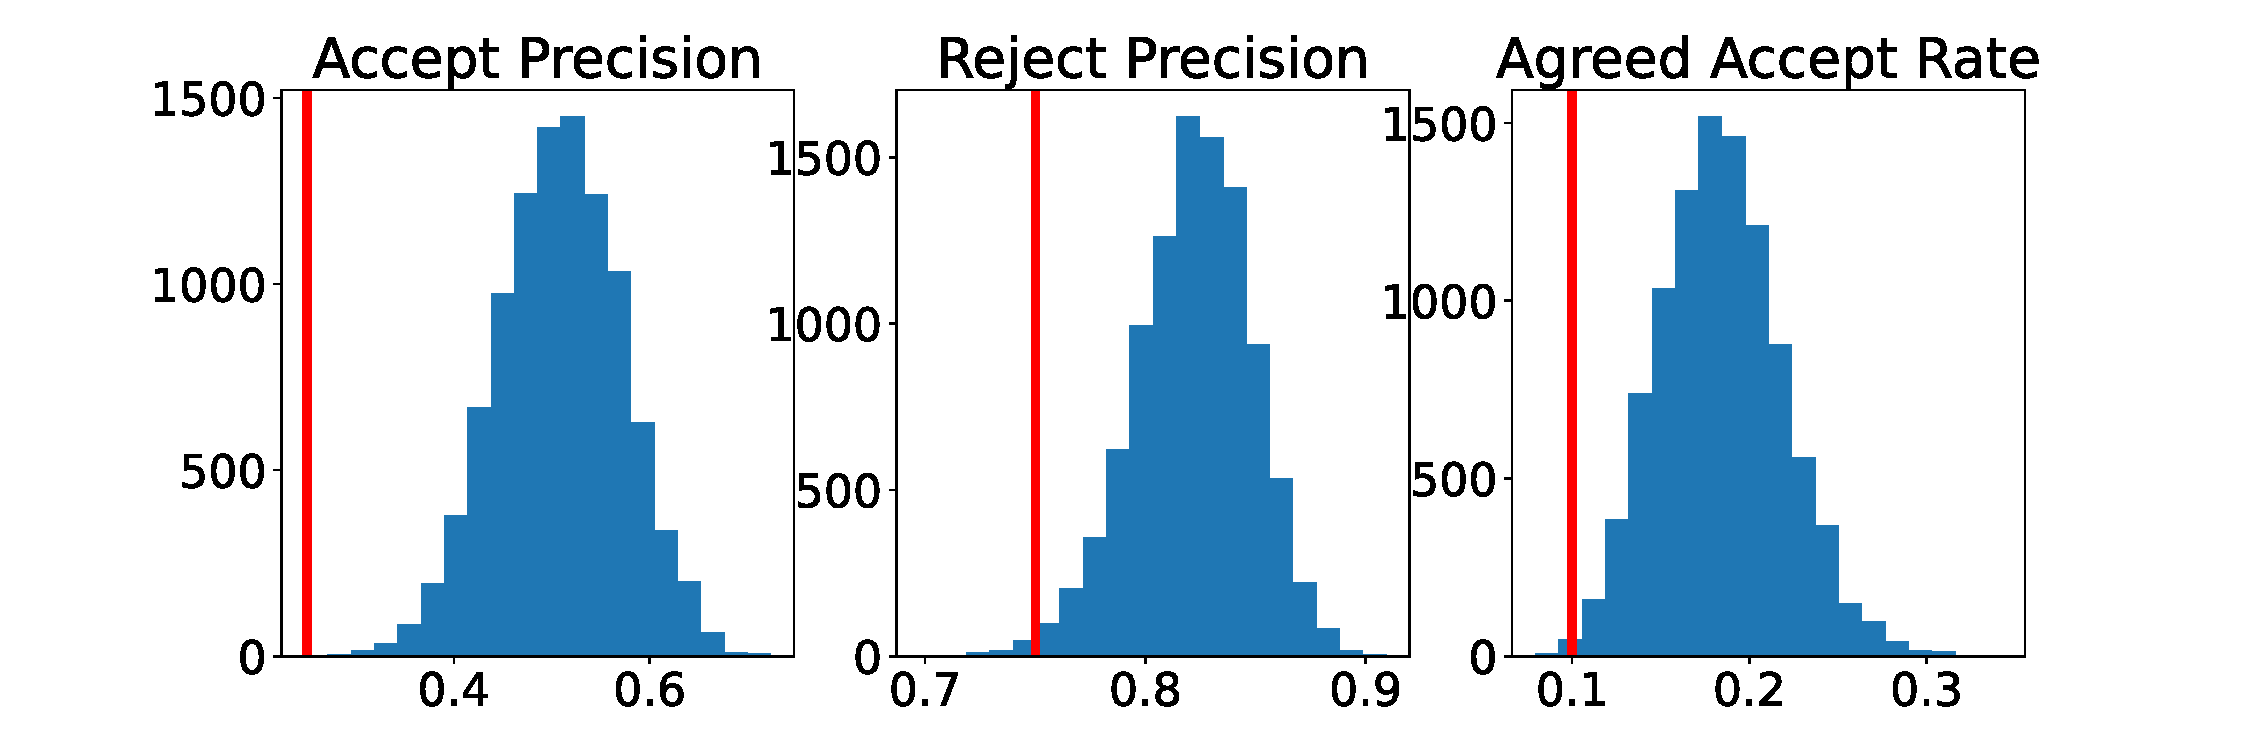
\includegraphics[width=0.90\textwidth]{https://inverseprobability.com/talks/slides/diagrams//neurips/random-committee-outcomes-vs-true.pdf}


\caption{Different statistics for the random committee oucomes versus the observed committee outcomes.}
\label{random-committee-outcomes}
\end{figure}

\hypertarget{model-choice-and-prior-values}{%
\subsubsection{Model Choice and Prior
Values}\label{model-choice-and-prior-values}}

In the analysis above we've minimized the modeling choices: we made use
of a Bayesian analysis to capture the uncertainty in counts that can be
arising from statistical sampling error. To this end we chose an
uninformative prior over these probabilities. However, one might argue
that the prior should reflect something more about the underlying
experimental structure: for example we \emph{know} that if the
committees made their decisions independently it is unlikely that we'd
obtain an inconsistency figure much greater than 37.5\% because that
would require committees to explicitly collude to make inconsistent
decisions: the random conference is the worst case. Due to the accept
rate, we also expect a larger number of reject decisions than reject.
This also isn't captured in our prior. Such questions actually move us
into the realms of modeling the process, rather then performing a
sensitivity analysis. However, if we wish to model the decision process
as a whole we have a lot more information available, and we should make
use of it. The analysis above is intended to exploit our randomized
experiment to explore how inconsistent we expect two committees to be.
It focusses on that single question, it doesn't attempt to give answers
on what the reasons for that inconsistency are and how it may be
reduced. The additional maths was needed only to give a sense of the
uncertainty in the figures. That uncertainty arises due to the limited
number of papers in the experiment.

\hypertarget{conclusion}{%
\subsection{Conclusion}\label{conclusion}}

\begin{flushright}
[\href{https://github.com/lawrennd/talks/edit/gh-pages/_neurips/includes/neurips-experiment-conclusion.md}{edit}]
\end{flushright}

Under the simple model we have outlined, we can be confident that there
is inconsistency between two independent committees, but the level of
inconsistency is much less than we would find for a random committee. If
we accept that the bias introduced by the Area Chairs knowing when they
were dealing with duplicates was minimal, then if we were to revisit the
NIPS 2014 conference with an independent committee then we would expect
between \textbf{38\% and 64\% of the presented papers to be the same}.
If the conference was run at random, then we would only expect 25\% of
the papers to be the same.

It's apparent from comments and speculation about what these results
mean, that some people might be surprised by the size of this figure.
However, it only requires a little thought to see that this figure is
likely to be large for any highly selective conference if there is even
a small amount of inconsistency in the decision making process. This is
because once the conference has chosen to be `highly selective' then
because by definition only a small percentage of papers are to be
accepted. Now if we think of a type I error as accepting a paper which
should be rejected, such errors are easier to make because by definition
many more papers should be rejected. Type II errors (rejecting a paper
that should be accepted) are less likely becaue (by setting the accept
rate low) there are fewer papers that should be accepted in the first
place. When there is a difference of opinion between reviewers, it does
seem that many of the arugments can be distilled down to (a subjective
opinion) about whether controlling for type I or type II errors is more
important. Further, normally when discussing type I and type II errors
we believe that the underlying system of study is genuinely binary:
e.g.~diseased or not diseased. However, for conferences the
accept/reject boundary is not a clear separation point, there is a
continuum (or spectrum) of paper quality (as there also is for some
diseases). And the decision boundary often falls in a region of very
high density.

\hypertarget{discussion}{%
\subsection{Discussion}\label{discussion}}

\begin{flushright}
[\href{https://github.com/lawrennd/talks/edit/gh-pages/_neurips/includes/neurips-experiment-discussion.md}{edit}]
\end{flushright}

As with any decision making process there are two types of errors we can
make, a type I error is accepting a paper that should be rejected. A
type II error is rejecting a paper that shoudl be accepted. Many
discussions about reviewing could be summarised as subjective opinions
about whether controlling for type I or type II is more important. When
accept rates are low type I errors are \emph{much more common}.

Many of these discussions seem to be based on a premise that there's an
underlying boundary of acceptable/non-acceptable papers. But for
conferences it is clear there is no separation point, there is a
spectrum of paper quality.

\hypertarget{thanks}{%
\subsection{Thanks!}\label{thanks}}

For more information on these subjects and more you might want to check
the following resources.

\begin{itemize}
\tightlist
\item
  twitter: \href{https://twitter.com/lawrennd}{@lawrennd}
\item
  podcast: \href{http://thetalkingmachines.com}{The Talking Machines}
\item
  newspaper:
  \href{http://www.theguardian.com/profile/neil-lawrence}{Guardian
  Profile Page}
\item
  blog:
  \href{http://inverseprobability.com/blog.html}{http://inverseprobability.com}
\end{itemize}

%%%%%%%%%%  End Body  %%%%%%%%%%

\bibliography{../lawrence.bib,../other.bib,../zbooks.bib}

\end{document}
